\documentclass[border=10pt]{standalone}
\usepackage{pgfplots}
\pgfplotsset{compat=1.18}
\begin{document}
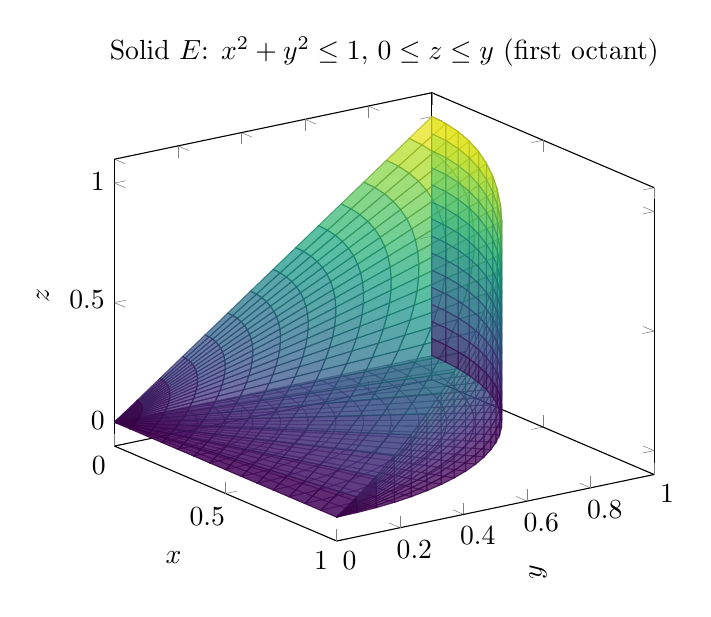
\begin{tikzpicture}
\begin{axis}[
    view={55}{22},
    axis lines=box,
    xlabel={$x$}, ylabel={$y$}, zlabel={$z$},
    title={Solid $E$: $x^2+y^2\le 1$, $0\le z\le y$ (first octant)},
    domain=0:90,
    y domain=0:1,
    samples=25, samples y=15,
    colormap/viridis,
]
% Bottom face z = 0 over the quarter disk
\addplot3[surf, shader=faceted, opacity=0.45]
    ({cos(x)*y}, {sin(x)*y}, {0});
% Top face z = y over the quarter disk
\addplot3[surf, shader=faceted, opacity=0.75]
    ({cos(x)*y}, {sin(x)*y}, {sin(x)*y});
% Cylinder wall x^2+y^2=1, 0<=z<=y
\addplot3[surf, shader=faceted, opacity=0.6, domain=0:90, y domain=0:1]
    ({cos(x)}, {sin(x)}, {y*sin(x)});
\end{axis}
\end{tikzpicture}
\end{document}
